\chapter{Low-Fidelity Prototypes}
\label{chapter:Mockups}

Low-fidelity prototypes are basic, early-stage representations of a product’s interface. They are used to rapidly explore design ideas, test usability, and gather feedback before progressing to high-fidelity design and full development. \\

\section{Mockups}

For the \ac{splash} project, \textbf{Figma} was initially used as a collaborative tool for brainstorming and sketching early interface concepts. Its real-time collaboration features allowed team members to quickly share and iterate on ideas during the early design phase, as illustrated in the figures below:

\begin{figure}[H]
    \centering
    \begin{subfigure}{0.48\textwidth}
        \centering
        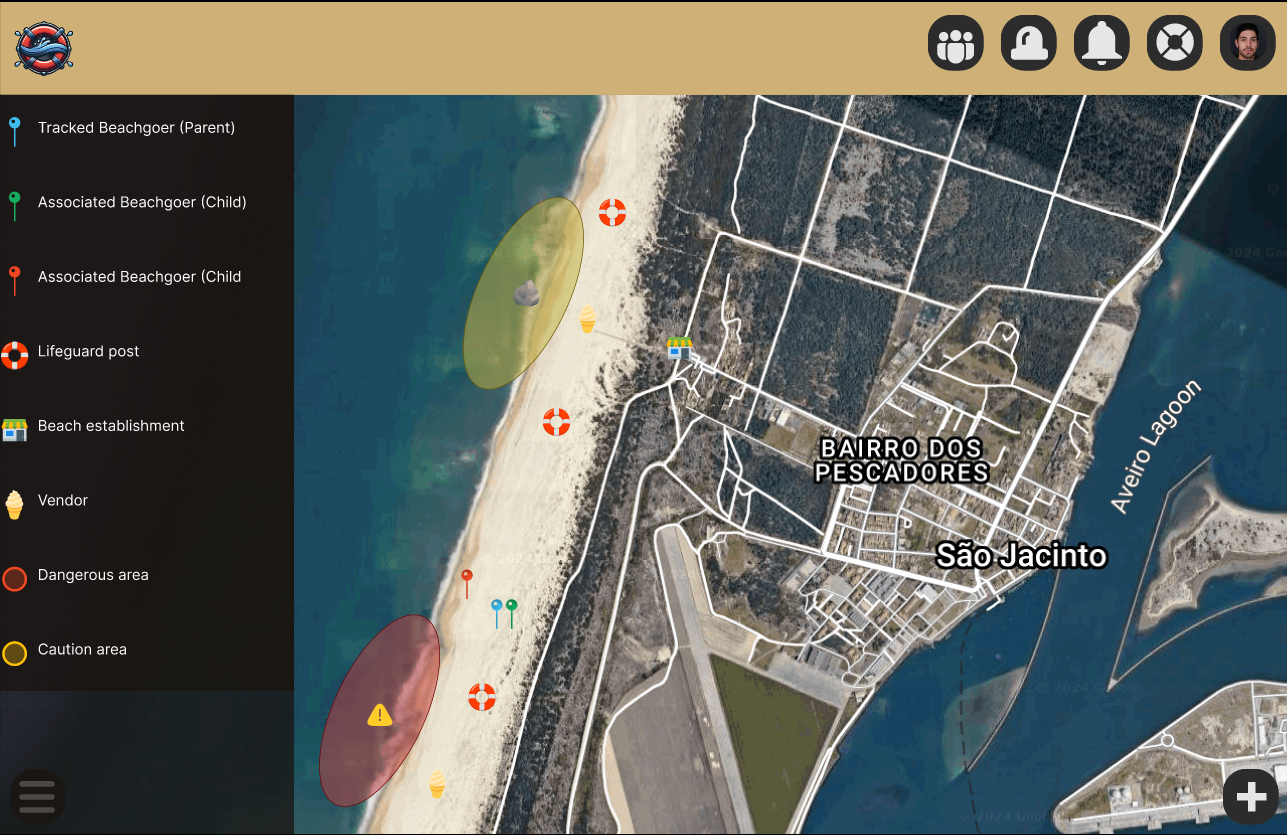
\includegraphics[width=\linewidth]{figs/Mockups/MAP_index.png}
        \caption{\ac{splash} mockup: Index menu open on map}
        \label{fig:figma_map_index}
    \end{subfigure}
    \hfill
    \begin{subfigure}{0.48\textwidth}
        \centering
        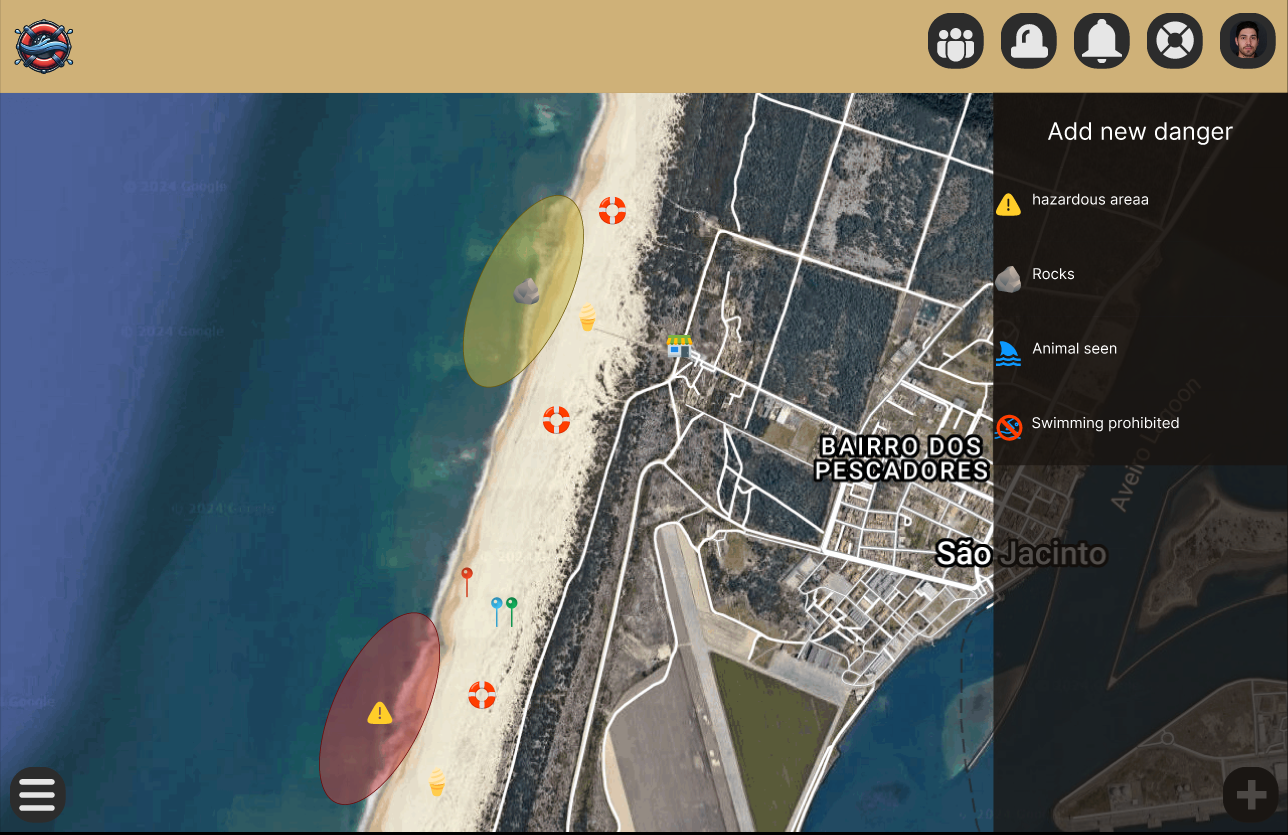
\includegraphics[width=\linewidth]{figs/Mockups/MAP_add1.png}
        \caption{\ac{splash} mockup: Add hazard menu open on map}
        \label{fig:figma_hazard_menu}
    \end{subfigure}
    \caption{Early-stage design brainstorming using Figma. For a more detailed and interactive view, access the full project here: \href{https://www.figma.com/design/73s1I8BXApUguw381t41PD/SPLASH?node-id=9-87&t=9a5nUxewcWEebZo4-1}{\ac{splash} Figma Design}.}
    \label{fig:figma_prototype}
\end{figure}

Once the general layout and structure of the interface had been agreed upon, the team transitioned to \textbf{Microsoft PowerPoint} to develop all mockups in detail. PowerPoint was chosen due to its familiarity among all team members and its ease of use for quickly assembling and customizing interface elements. The mockups were collaboratively developed using the team’s shared \textbf{OneDrive} workspace, which ensured effective version control and feedback. \\
Below are several images showcasing the final low-fidelity prototypes developed using \textbf{Microsoft PowerPoint}:\\

As illustrated (Figure \ref{fig:interactive-map}), the main feature of \ac{splash} is an interactive map that allows users to navigate and access detailed beach information. At this stage, the interactive map enables users to view their GPS location, the positions of lifeguard posts, the real-time locations of individual lifeguards, as well as the locations of restrooms, beach bars, restaurants, and mobile vendors.

\begin{figure}[H]
    \centering
    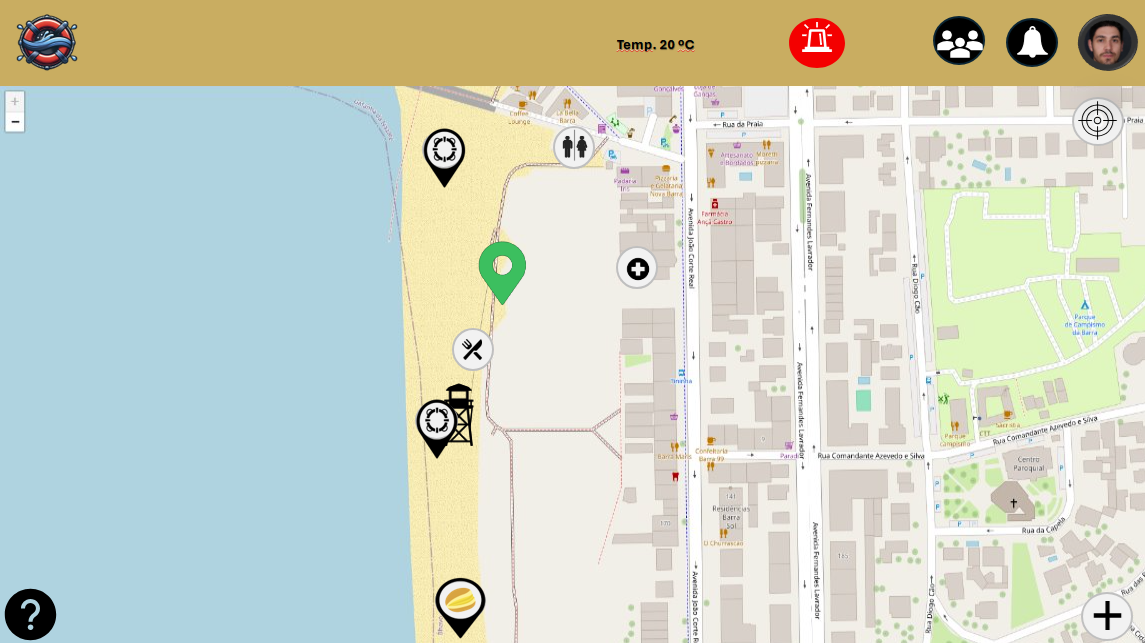
\includegraphics[width=13cm,height=7cm]{figs/Mockups/ppt-mockups-maps.png}
    \caption{\ac{splash} mockup: Interactive Map}
    \label{fig:interactive-map}
\end{figure}

Additionally, the map features a variety of menus and pop-ups (Figure \ref{fig:ppt-map-menus-popups}) that appear when users click on specific icons. These include detailed information and editing options for guard posts, general information about lifeguards, and menus for bars and restaurants. Users can also consult a legend for icon clarification and report new hazards they encounter on the beach.

\begin{figure}[H]
    \centering
    \begin{subfigure}{0.48\textwidth}
    \centering
    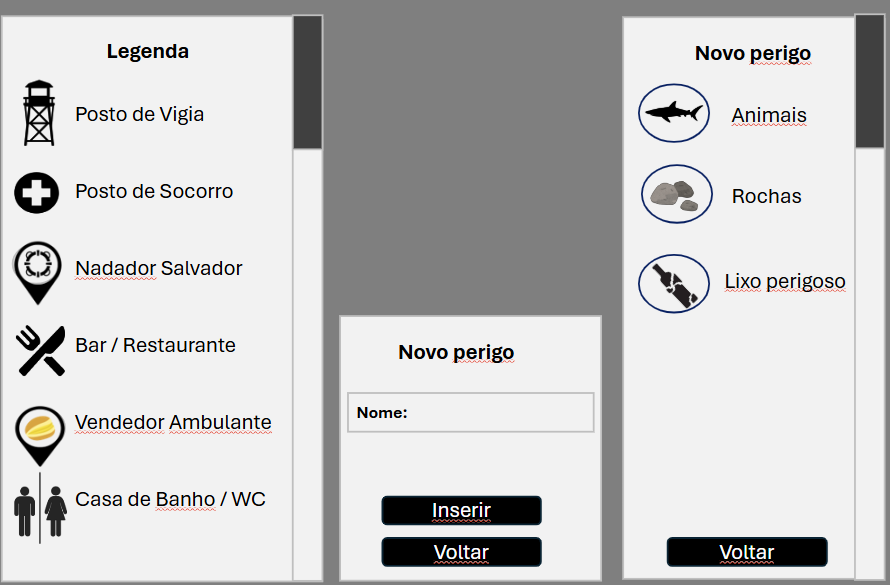
\includegraphics[width=\linewidth]{figs/Mockups/ppt-mockups-menus.png}
    \caption{\ac{splash} mockup: Interactive Map Menus}
    \label{fig:ppt-mockups-menus}
    \end{subfigure}
    \hfill
    \begin{subfigure}{0.48\textwidth}
    \centering
    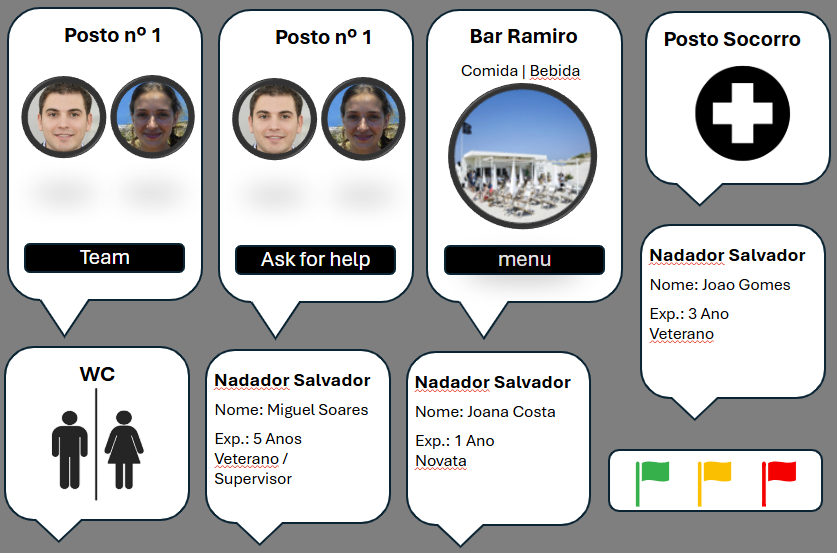
\includegraphics[width=\linewidth]{figs/Mockups/ppt-mockups-popups.png}
    \caption{\ac{splash} mockup: Interactive Map Pop-ups}
    \label{fig:ppt-mockups-popups}
    \end{subfigure}
    \caption{Examples of interactive menus and pop-ups in the SPLASH map prototype.}
    \label{fig:ppt-map-menus-popups}
\end{figure}

The application features dedicated menus for organizing teams and managing lifeguard assignments at each beach (Figure \ref{fig:ppt-map-team-management}). The beach teams menu (left) allows users to browse available beaches, search for specific teams, and view the number of members in each team. Users can easily create new teams or delete entire beaches as needed. The beach guard posts menu (right) provides a detailed view of team members assigned to a specific post, including their names, years of experience, and relevant roles or certifications. This interface supports quick editing of team compositions.


\begin{figure}[H]
    \centering
    \begin{subfigure}{0.48\textwidth}
    \centering
    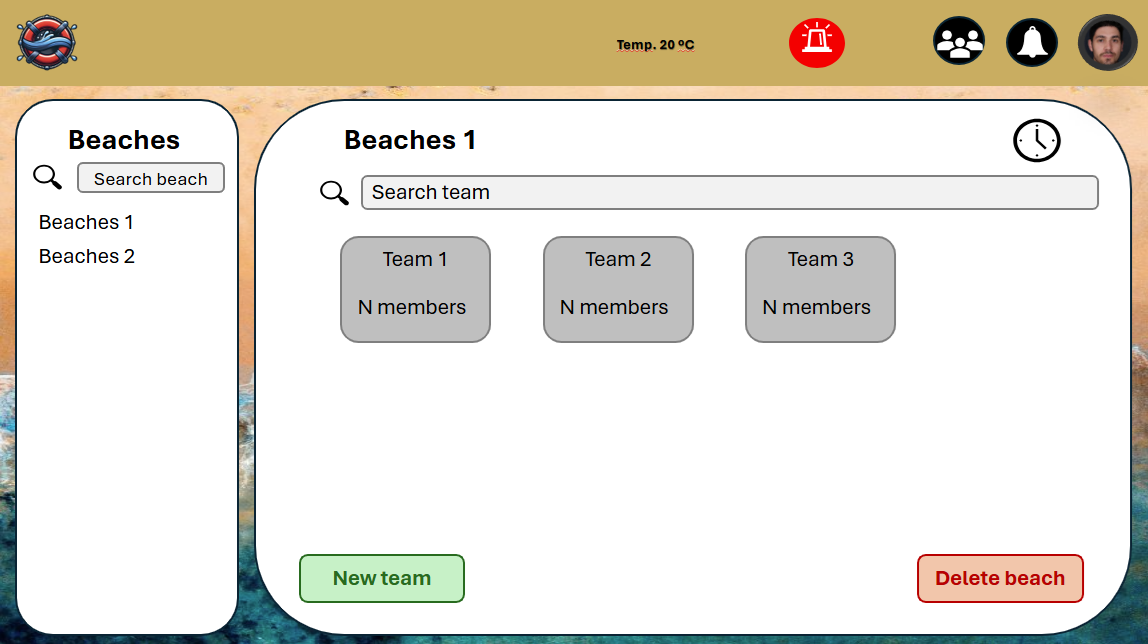
\includegraphics[width=\linewidth]{figs/Mockups/ppt-mockups-beach-teams.png}
    \caption{\ac{splash} mockup: Beach teams menu}
    \label{fig:ppt-mockups-teams}
    \end{subfigure}
    \hfill
    \begin{subfigure}{0.48\textwidth}
    \centering
    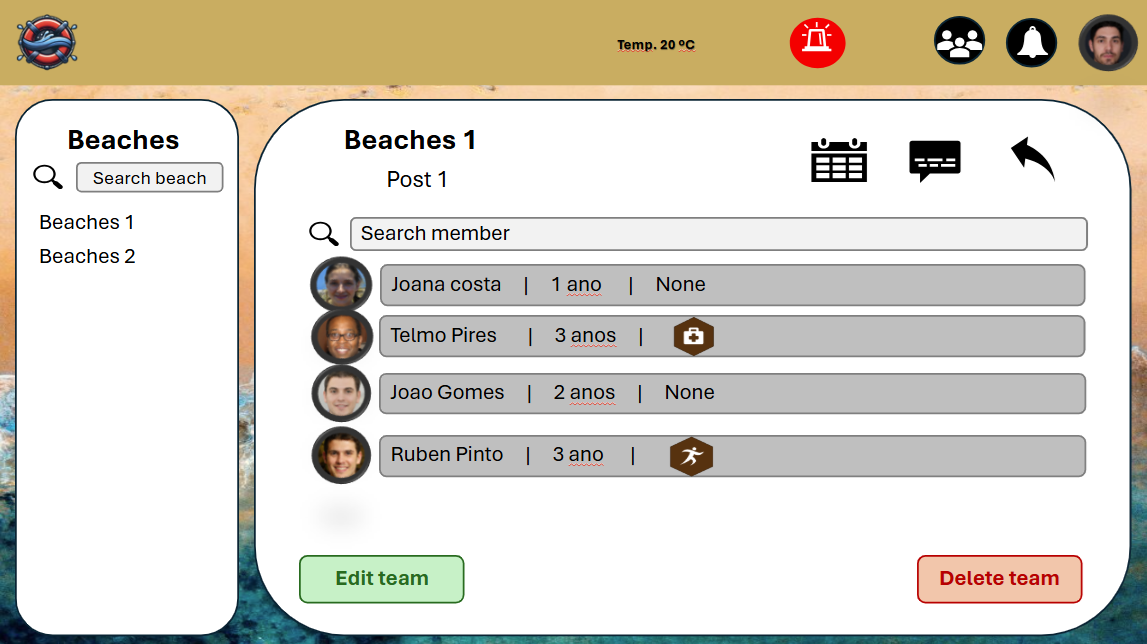
\includegraphics[width=\linewidth]{figs/Mockups/ppt-mockups-posts.png}
    \caption{\ac{splash}: Beach guard posts menu}
    \label{fig:ppt-mockups-posts}
    \end{subfigure}
    \caption{some caption...}
    \label{fig:ppt-map-team-management}
\end{figure}

The application also provides dedicated interfaces for managing beach safety operations (Figure \ref{fig:ppt-map-team-management}). On the left, users can access a comprehensive hazard history for each beach, displaying a chronological list of recorded incidents with details such as date, time, hazard type, affected post, and current status. This facilitates efficient monitoring and resolution of safety issues. On the right, the scheduling menu allows managers to organize and visualize weekly staff assignments for each beach guard post. Users can filter by member, day, and shift times, ensuring optimal coverage and clear oversight of lifeguard duties throughout the week.

\begin{figure}[H]
    \centering
    \begin{subfigure}{0.48\textwidth}
    \centering
    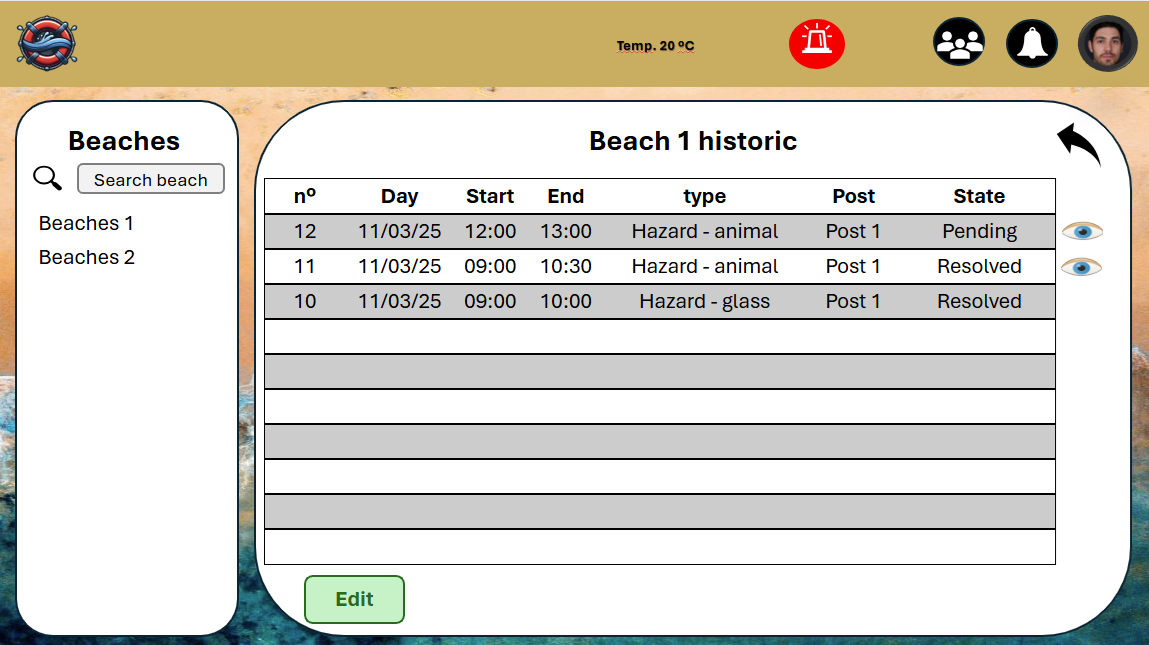
\includegraphics[width=\linewidth]{figs/Mockups/ppt-mockups-beach-history.png}
    \caption{\ac{splash}: Beach's hazard history }
    \label{fig:ppt-mockups-hazard-history}
    \end{subfigure}
    \hfill
    \begin{subfigure}{0.48\textwidth}
    \centering
    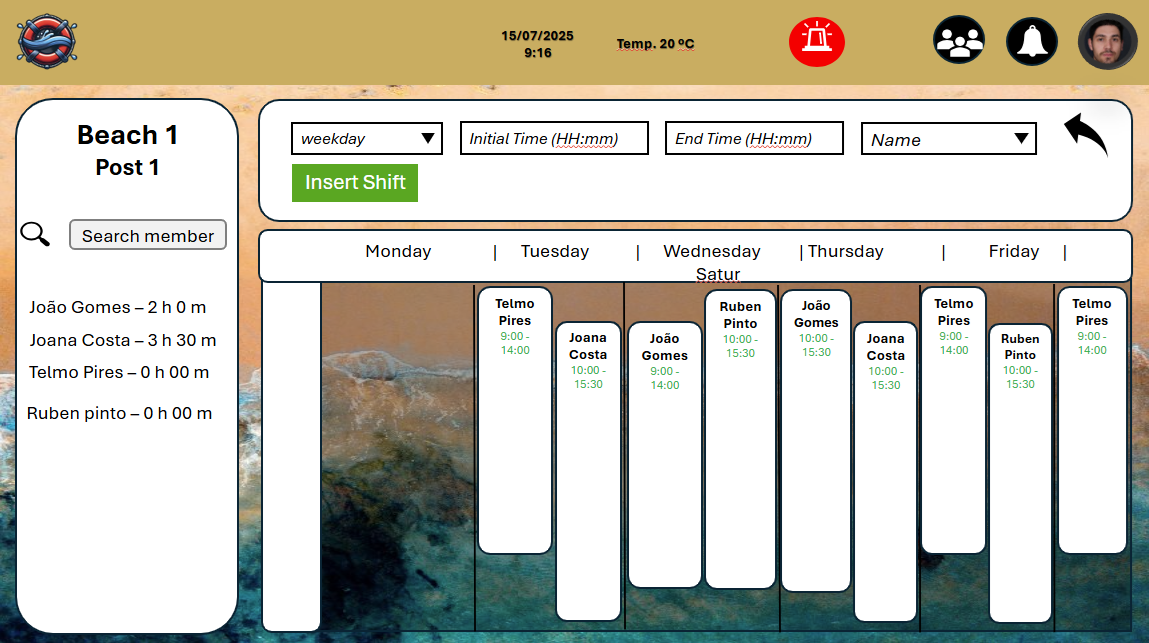
\includegraphics[width=\linewidth]{figs/Mockups/ppt-mockups-schedule.png}
    \caption{\ac{splash}: Beach guard posts schedules }
    \label{fig:ppt-mockups-team-schedule}
    \end{subfigure}
    \caption{some caption...}
    \label{fig:ppt-map-team-management}
\end{figure}

Furthermore, PowerPoint enabled the team to print and cut out each interface screen, which was essential for conducting hands-on usability testing sessions, discussed in chapter \ref{chapter:Usability}. This practical approach allowed users to simulate interactions and provide valuable feedback during early development stages.\\
A complete version of the mockups is available online at: \url{https://github.com/SPLASHub/SplashDocumentation}. \\

These low-fidelity prototypes played a central role in the early design validation process. Not only did they enable quick iterations and collective design decisions, but they also formed the foundation for the usability testing procedures described in the following chapter.

\noindent In particular, the printed and cut-out mockups were instrumental in simulating realistic interactions through the Wizard of Oz technique, providing valuable insights into how users engaged with the interface concepts and navigation flow.

To ensure that the \ac{splash} system aligns with user needs and expectations, a usability evaluation was conducted using the low-fidelity prototypes presented in Chapter~\ref{chapter:Mockups}. This process was designed to identify usability issues at an early stage and to guide subsequent improvements prior to further development.

\section{Methods}

\subsection{Wizard of Oz Approach}
The Wizard of Oz approach was utilized as a prototyping technique in which users interacted with what appeared to be a functioning system, while all functionalities were operated by a human behind the scenes. This method enabled the simulation of key features of \ac{splash} and facilitated the observation of authentic user interactions.

\subsection{Usability Testing Procedure}
\begin{itemize}
    \item \textbf{Participants:} Five individuals participated in the usability tests, representing typical end-users of the \ac{splash} system. This sample size is considered sufficient for identifying the majority of usability issues in formative evaluations.
    \item \textbf{Testing Environment:} System responses were simulated by the test facilitator as required, following the Wizard of Oz methodology.
    \item \textbf{Tasks:} Participants were instructed to complete a series of representative tasks, including navigating the interactive map, locating lifeguard posts, and reporting a beach hazard.
    \item \textbf{Observation and Think-Aloud Protocol:} User actions were observed throughout the testing process, and participants were encouraged to verbalize their thoughts, decisions, and any encountered difficulties, following the think-aloud method.
    \item \textbf{Post-Test Feedback:} Upon completion of the tasks, participants provided feedback through a brief interview and completed a usability questionnaire (\ac{sus}).
\end{itemize}

\section{Evaluation Objective}
The primary objective of this usability evaluation is to achieve a System Usability Scale (\acf{sus}) score of at least 70\%, which is recognized as a benchmark for acceptable usability in interactive systems.

\section{Expected Results}
Based on established usability testing practices, the evaluation is expected to identify:
\begin{itemize}
    \item Areas of confusion or difficulty within the interface;
    \item Features that are intuitive and support user goals;
    \item Suggestions for improvement provided by participants;
    \item An overall usability score (derived from the \ac{sus} questionnaire) to benchmark the prototype’s effectiveness.
\end{itemize}

\section{Summary}
The usability evaluation, utilizing the Wizard of Oz approach and structured user testing, provided valuable insights into the strengths and weaknesses of the \ac{splash} prototype, informing subsequent design iterations and supporting the development of a user-centered final system.

\begin{figure}[H]
    \centering
    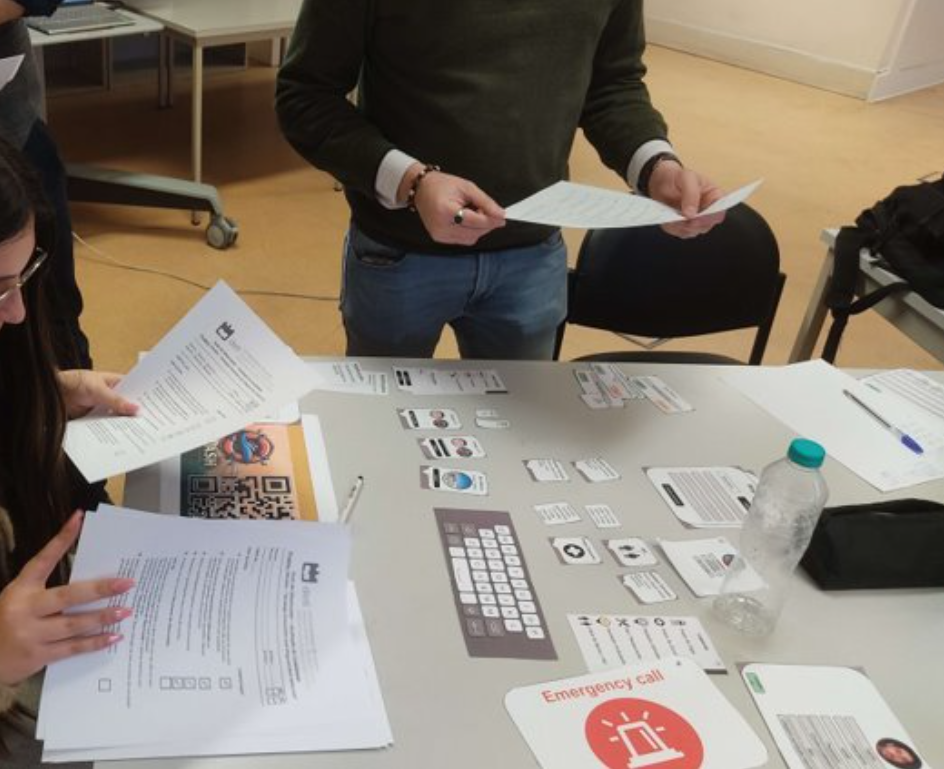
\includegraphics[width=13cm,height=10cm]{figs/mockup-tests.png}
    \caption{\ac{splash}: Photograph captured during a usability testing session with users}
    \label{fig:usability-testing}
\end{figure}

\section{Conclusion}

These low-fidelity prototypes enabled quick iterations and collective design decisions, forming the foundation for the usability testing procedures described in the following chapter. The printed and cut-out mockups were instrumental in simulating realistic interactions through the Wizard of Oz technique, providing valuable insights into how users engaged with the interface concepts and navigation flow.